\documentclass[14pt]{extbook}
\usepackage{multicol, enumerate, enumitem, hyperref, color, soul, setspace, parskip, fancyhdr} %General Packages
\usepackage{amssymb, amsthm, amsmath, latexsym, units, mathtools} %Math Packages
\everymath{\displaystyle} %All math in Display Style
% Packages with additional options
\usepackage[headsep=0.5cm,headheight=12pt, left=1 in,right= 1 in,top= 1 in,bottom= 1 in]{geometry}
\usepackage[usenames,dvipsnames]{xcolor}
\usepackage{dashrule}  % Package to use the command below to create lines between items
\newcommand{\litem}[1]{\item#1\hspace*{-1cm}\rule{\textwidth}{0.4pt}}
\pagestyle{fancy}
\lhead{Progress Quiz 7}
\chead{}
\rhead{Version B}
\lfoot{4173-5738}
\cfoot{}
\rfoot{Spring 2021}
\begin{document}

\begin{enumerate}
\litem{
Construct the lowest-degree polynomial given the zeros below. Then, choose the intervals that contain the coefficients of the polynomial in the form $ax^3+bx^2+cx+d$.\[ -6, \frac{7}{2}, \text{ and } -7 \]\begin{enumerate}[label=\Alph*.]
\item \( a \in [1, 3], b \in [4, 18], c \in [-85, -74], \text{ and } d \in [-296, -290] \)
\item \( a \in [1, 3], b \in [19, 24], c \in [-10, -5], \text{ and } d \in [-296, -290] \)
\item \( a \in [1, 3], b \in [-21, -18], c \in [-10, -5], \text{ and } d \in [290, 297] \)
\item \( a \in [1, 3], b \in [19, 24], c \in [-10, -5], \text{ and } d \in [290, 297] \)
\item \( a \in [1, 3], b \in [-9, -4], c \in [-96, -85], \text{ and } d \in [290, 297] \)

\end{enumerate} }
\litem{
Which of the following equations \textit{could} be of the graph presented below?
\begin{center}
    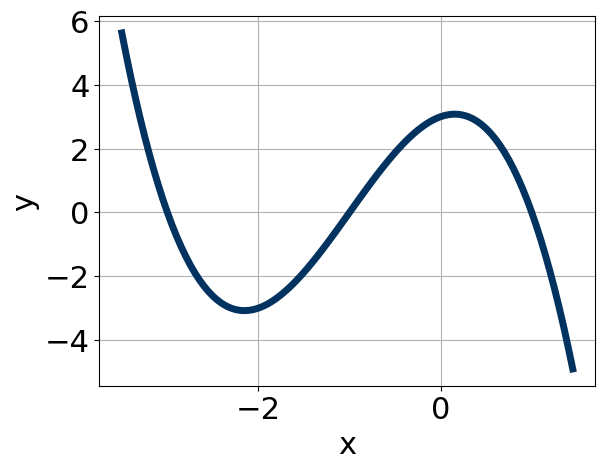
\includegraphics[width=0.5\textwidth]{../Figures/polyGraphToFunctionB.png}
\end{center}
\begin{enumerate}[label=\Alph*.]
\item \( -3(x + 4)^{4} (x + 2)^{5} (x + 3)^{5} \)
\item \( -7(x + 4)^{9} (x + 2)^{10} (x + 3)^{5} \)
\item \( 10(x + 4)^{6} (x + 2)^{5} (x + 3)^{6} \)
\item \( -4(x + 4)^{4} (x + 2)^{4} (x + 3)^{11} \)
\item \( 18(x + 4)^{4} (x + 2)^{7} (x + 3)^{5} \)

\end{enumerate} }
\litem{
Describe the zero behavior of the zero $x = -4$ of the polynomial below.\[ f(x) = 7(x - 8)^{5}(x + 8)^{2}(x + 4)^{10}(x - 4)^{5} \]\begin{enumerate}[label=\Alph*.]
\begin{multicols}{2}\item 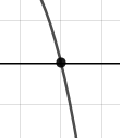
\includegraphics[width = 0.3\textwidth]{../Figures/polyZeroBehaviorAB.png}\item 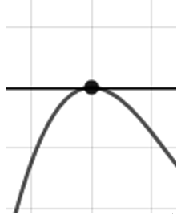
\includegraphics[width = 0.3\textwidth]{../Figures/polyZeroBehaviorBB.png}\item 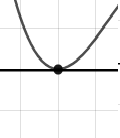
\includegraphics[width = 0.3\textwidth]{../Figures/polyZeroBehaviorCB.png}\item 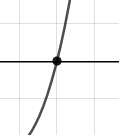
\includegraphics[width = 0.3\textwidth]{../Figures/polyZeroBehaviorDB.png}\end{multicols}\item None of the above.
\end{enumerate} }
\litem{
Construct the lowest-degree polynomial given the zeros below. Then, choose the intervals that contain the coefficients of the polynomial in the form $x^3+bx^2+cx+d$.\[ 4 - 4 i \text{ and } 4 \]\begin{enumerate}[label=\Alph*.]
\item \( b \in [-15, -11], c \in [61, 66], \text{ and } d \in [-132, -126] \)
\item \( b \in [4, 17], c \in [61, 66], \text{ and } d \in [124, 131] \)
\item \( b \in [-3, 6], c \in [-4, 2], \text{ and } d \in [-19, -15] \)
\item \( b \in [-3, 6], c \in [-8, -5], \text{ and } d \in [16, 20] \)
\item \( \text{None of the above.} \)

\end{enumerate} }
\litem{
Construct the lowest-degree polynomial given the zeros below. Then, choose the intervals that contain the coefficients of the polynomial in the form $ax^3+bx^2+cx+d$.\[ -2, \frac{-3}{5}, \text{ and } \frac{1}{3} \]\begin{enumerate}[label=\Alph*.]
\item \( a \in [9, 26], b \in [-32, -20], c \in [-11, -8], \text{ and } d \in [2, 11] \)
\item \( a \in [9, 26], b \in [31, 43], c \in [0, 11], \text{ and } d \in [2, 11] \)
\item \( a \in [9, 26], b \in [-48, -38], c \in [29, 33], \text{ and } d \in [-6, -3] \)
\item \( a \in [9, 26], b \in [31, 43], c \in [0, 11], \text{ and } d \in [-6, -3] \)
\item \( a \in [9, 26], b \in [-34, -33], c \in [0, 11], \text{ and } d \in [2, 11] \)

\end{enumerate} }
\litem{
Describe the zero behavior of the zero $x = 5$ of the polynomial below.\[ f(x) = 4(x - 5)^{2}(x + 5)^{5}(x + 8)^{6}(x - 8)^{9} \]\begin{enumerate}[label=\Alph*.]
\begin{multicols}{2}\item 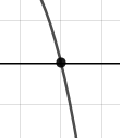
\includegraphics[width = 0.3\textwidth]{../Figures/polyZeroBehaviorCopyAB.png}\item 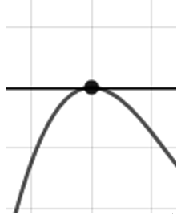
\includegraphics[width = 0.3\textwidth]{../Figures/polyZeroBehaviorCopyBB.png}\item 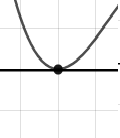
\includegraphics[width = 0.3\textwidth]{../Figures/polyZeroBehaviorCopyCB.png}\item 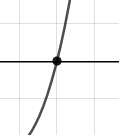
\includegraphics[width = 0.3\textwidth]{../Figures/polyZeroBehaviorCopyDB.png}\end{multicols}\item None of the above.
\end{enumerate} }
\litem{
Describe the end behavior of the polynomial below.\[ f(x) = -7(x + 8)^{4}(x - 8)^{9}(x + 6)^{5}(x - 6)^{5} \]\begin{enumerate}[label=\Alph*.]
\begin{multicols}{2}\item 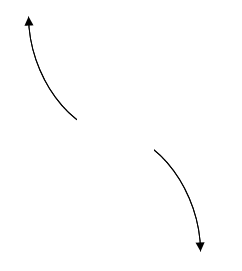
\includegraphics[width = 0.3\textwidth]{../Figures/polyEndBehaviorCopyAB.png}\item 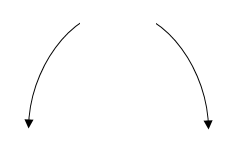
\includegraphics[width = 0.3\textwidth]{../Figures/polyEndBehaviorCopyBB.png}\item 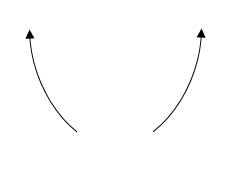
\includegraphics[width = 0.3\textwidth]{../Figures/polyEndBehaviorCopyCB.png}\item 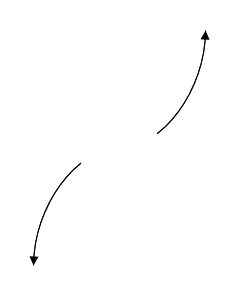
\includegraphics[width = 0.3\textwidth]{../Figures/polyEndBehaviorCopyDB.png}\end{multicols}\item None of the above.
\end{enumerate} }
\litem{
Describe the end behavior of the polynomial below.\[ f(x) = 6(x + 9)^{4}(x - 9)^{9}(x + 5)^{5}(x - 5)^{7} \]\begin{enumerate}[label=\Alph*.]
\begin{multicols}{2}\item 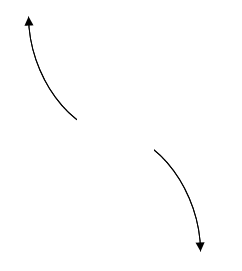
\includegraphics[width = 0.3\textwidth]{../Figures/polyEndBehaviorAB.png}\item 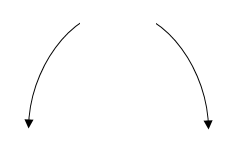
\includegraphics[width = 0.3\textwidth]{../Figures/polyEndBehaviorBB.png}\item 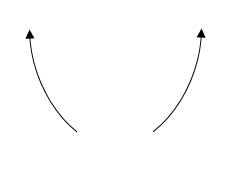
\includegraphics[width = 0.3\textwidth]{../Figures/polyEndBehaviorCB.png}\item 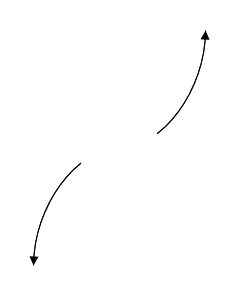
\includegraphics[width = 0.3\textwidth]{../Figures/polyEndBehaviorDB.png}\end{multicols}\item None of the above.
\end{enumerate} }
\litem{
Which of the following equations \textit{could} be of the graph presented below?
\begin{center}
    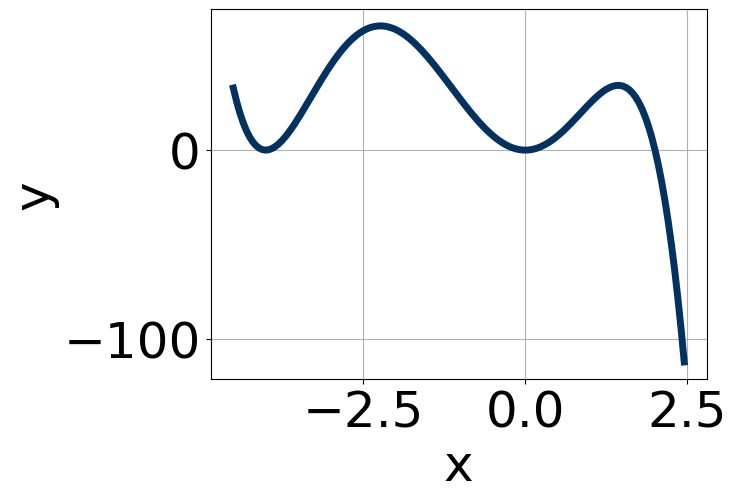
\includegraphics[width=0.5\textwidth]{../Figures/polyGraphToFunctionCopyB.png}
\end{center}
\begin{enumerate}[label=\Alph*.]
\item \( 20(x + 3)^{6} (x + 2)^{6} (x + 1)^{5} \)
\item \( 11(x + 3)^{8} (x + 2)^{5} (x + 1)^{7} \)
\item \( -11(x + 3)^{6} (x + 2)^{6} (x + 1)^{7} \)
\item \( 18(x + 3)^{8} (x + 2)^{7} (x + 1)^{10} \)
\item \( -14(x + 3)^{8} (x + 2)^{4} (x + 1)^{10} \)

\end{enumerate} }
\litem{
Construct the lowest-degree polynomial given the zeros below. Then, choose the intervals that contain the coefficients of the polynomial in the form $x^3+bx^2+cx+d$.\[ 5 - 5 i \text{ and } 3 \]\begin{enumerate}[label=\Alph*.]
\item \( b \in [-16, -9], c \in [79, 86], \text{ and } d \in [-157, -147] \)
\item \( b \in [-8, 10], c \in [2, 7], \text{ and } d \in [-19, -11] \)
\item \( b \in [10, 14], c \in [79, 86], \text{ and } d \in [149, 151] \)
\item \( b \in [-8, 10], c \in [-9, -2], \text{ and } d \in [12, 16] \)
\item \( \text{None of the above.} \)

\end{enumerate} }
\end{enumerate}

\end{document}